\documentclass{article}
\usepackage[utf8]{inputenc}
\usepackage[T1]{fontenc}
\usepackage[spanish]{babel}
\usepackage[hidelinks]{hyperref}
\usepackage{graphicx}
\usepackage{titling}
\usepackage{float}
\usepackage{longtable}
\usepackage[text={18cm,21cm},centering]{geometry}
\usepackage{hyperref} \hypersetup{ colorlinks=true, linkcolor=blue, filecolor=magenta,
urlcolor=blue, }
\usepackage{listings}
\usepackage{xcolor}
\usepackage{booktabs}



% Definir colores adicionales si es necesario
\definecolor{gray}{rgb}{0.5, 0.5, 0.5}
\definecolor{lightgray}{rgb}{0.9, 0.9, 0.9}
\definecolor{green}{rgb}{0, 0.5, 0}
\definecolor{blue}{rgb}{0, 0, 1}
\definecolor{red}{rgb}{1, 0, 0}

\lstdefinestyle{mystyle}{
    backgroundcolor=\color{white},   
    commentstyle=\color{green},
    keywordstyle=\color{blue},
    numberstyle=\tiny\color{gray},
    stringstyle=\color{red},
    basicstyle=\ttfamily\footnotesize,
    breakatwhitespace=false,         
    breaklines=true,                 
    captionpos=b,                    
    keepspaces=true,                 
    numbers=left,                    
    numbersep=5pt,                  
    showspaces=false,                
    showstringspaces=false,
    showtabs=false,                  
    tabsize=2
}

\lstset{style=mystyle}


\begin{document}


\begin{titlepage}
    \centering
    {\bfseries\LARGE Universidad de La Habana \par}
    \vspace{1cm}
    {\scshape\Large Facultad de Matemática y Computación \par}
    \vspace{3cm}
    {\scshape\Huge Predicción de Problemas de Codeforces\par}
    \vfill
    
    {\Large Juan Carlos Espinosa Delgado C-411 \par}
    {\Large Raudel Alejandro Gómez Molina C-411 \par}
    {\Large Alex Sierra Alcalá C-411 \par}
    {\Large Yoan René Ramos Corrales C-412 \par}
    \vfill
    {\href{https://github.com/ARJ-Code/codeforce-tag-predictor}{Proyecto en github} \par}
\end{titlepage}

\section{Introducción}

\subsection{Motivación}

La plataforma Codeforces es una herramienta fundamental en la comunidad de programación competitiva, diseñada
para desarrollar y entrenar habilidades de resolución de problemas. Los problemas en Codeforces no solo desafían
a los competidores, sino que también proporcionan una base sólida para aprender y aplicar diversos algoritmos y
estructuras de datos. Cada problema está asociado a una serie de categorías o etiquetas que ayudan a identificar
los tipos de algoritmos y técnicas necesarias para resolverlos. Pero este proceso suele estar muy apegado a la
a la solución final del ejercicio por lo que la correcta identificación de los tags suele ser un gran reto para los
competidores.

Es válido aclarar que la automatización de este proceso no es interés de la programación competitiva, ya que en estos
escenarios lo que se busca es el razonamiento lógico de los competidores, en este contexto si pudiera ser interesante
el desarrollo de un mecanismo de generación de problemas, pero este no es el objetivo de este proyecto.

Sin embargo la experimentación con la detección de tags en escenarios controlados como este, manteniéndonos en el entorno
de que esta tarea es útil para la posterior solución del problema pudiera servir de base para proponer mecanismo de detección
de tags en problemas reales orientados al campo de la generación de algoritmos.

\subsection{Problemática}

Cada problema en la plataforma Codeforces y un problema de programación competitiva en general cuenta primeramente con
un título y una descripción en la cual se plantea el objetivo y la problemática del mismo, este segundo componente del
problema es la principal fuente de interés para la detección de tags ya que estos se encuentran explícitos en forma de
lenguaje natural en dicha descripción.

Pero además de la descripción los problemas cuentan con una restricción de tiempo y espacio de memoria donde se deben
desenvolver los algoritmos que den solución al problema (un algoritmo correcto para todos los casos de prueba
que no este dentro de los límites establecidos no es considerado como solución). Ahora bien esta restricción también
influye en los tags del algoritmo ya el conjunto de tags del problema que satisfacen estas restricciones y la descripción
del problema será subconjunto del conjunto de tags solo asociados a la descripción.

Otra característica interesante que nos pudiera aportar información sobre la naturaleza del problema es analizar el
código de una solución aceptada del problema, ya que es posible identificar los tags asociados a dicho código y por
tanto un subconjunto de los tags del problema. Es importante analizar que con este enfoque solo podemos obtener un
subconjunto de los tags ya que un mismo problema puede tener multiples soluciones y cada solución puede tener asociada
distintos tipos de tags.

Por tanto como tenemos de por medio un problema asociado a lenguaje natural y actualmente no hay ningún método asociado
medianamente eficaz asociado a este campo que no lleve Machine Learning, la propuesta de la solución descrita en este
trabajo empleará algoritmos de Machine Learning los cuales iremos introduciendo a lo largo de este trabajo.

\subsection{Objetivos Generales y Específicos}

\subsubsection{Objetivos Generales}

El objetivo general de este proyecto es desarrollar un sistema automatizado utilizando técnicas de Machine Learning para detectar y asignar etiquetas (tags) a los problemas de programación en Codeforces.


\subsubsection{Objetivos Específicos}

\begin{itemize}
    \item \textbf{Recolección y Preprocesamiento de Datos:}
          \begin{itemize}
              \item Recolectar un conjunto representativo de problemas de Codeforces, incluyendo sus descripciones, restricciones de tiempo y memoria, y etiquetas existentes.
              \item Realizar el preprocesamiento del texto de las descripciones para normalizar y limpiar los datos, facilitando su análisis.
          \end{itemize}
          
    \item \textbf{Desarrollo del Modelo de Machine Learning:}
          \begin{itemize}
              \item Investigar y seleccionar algoritmos de Machine Learning apropiados para la tarea de clasificación de texto, como KNN, Naive Bayes, y redes neuronales.
              \item Entrenar varios modelos utilizando el conjunto de datos preprocesado, ajustando hiperparámetros para optimizar el rendimiento.
          \end{itemize}
          
    \item \textbf{Evaluación del Modelo:}
          \begin{itemize}
              \item Evaluar los modelos entrenados utilizando métricas de rendimiento como precisión, recall, F1-score y exactitud.
              \item Comparar los resultados de diferentes modelos para identificar el más eficaz en la detección de etiquetas.
              \item Comparar los resultados con un modelo de lenguaje (en este caso se usará Chat-GPT 3.5).
          \end{itemize}
          
    \item \textbf{Implementación y Prueba:}
          \begin{itemize}
              \item Implementar el modelo seleccionado en un entorno de prueba para evaluar su rendimiento en condiciones reales.
              \item Realizar pruebas adicionales para validar la consistencia y robustez del sistema en la asignación de etiquetas.
          \end{itemize}
          
    \item \textbf{Documentación y Propuesta de Mejora:}
          \begin{itemize}
              \item Documentar el proceso completo de desarrollo, incluyendo la recolección de datos, preprocesamiento, desarrollo del modelo, evaluación e implementación.
              \item Proponer mejoras y futuras líneas de investigación basadas en los resultados obtenidos y las limitaciones encontradas durante el desarrollo del proyecto.
          \end{itemize}
\end{itemize}

\subsubsection{Hipótesis}

\begin{itemize}
    \item \textbf{Hipótesis Principal:} Un modelo de Machine Learning bien entrenado puede detectar y asignar etiquetas (tags) a los problemas de programación de Codeforces con una precisión comparable a la de un humano experto.
    \item \textbf{Hipótesis Secundarias:}
          \begin{itemize}
              \item Los algoritmos de clasificación de texto basados en redes neuronales (como LSTM o Transformers) ofrecerán un mejor rendimiento en la detección de etiquetas en comparación con algoritmos más tradicionales como Naive Bayes o KNN.
              \item El análisis y utilización de las restricciones de tiempo y memoria, así como del código de soluciones aceptadas, pueden mejorar significativamente la precisión del modelo en la asignación de etiquetas.
          \end{itemize}
\end{itemize}

\subsubsection{Preguntas Científicas}

\begin{itemize}
    \item ¿Qué algoritmos de Machine Learning son más efectivos para la tarea de detección de etiquetas en problemas de programación competitiva?
    \item ¿Cómo influye la calidad y cantidad de los datos de entrenamiento en el rendimiento del modelo?
    \item ¿En qué medida las restricciones de tiempo y memoria impactan en la precisión de la detección de etiquetas?
    \item ¿Es posible mejorar la detección de etiquetas utilizando información adicional del código de soluciones aceptadas?
    \item ¿Cuáles son las principales limitaciones y desafíos al aplicar Machine Learning en la detección de etiquetas en problemas de programación competitiva?
\end{itemize}

\section{Análisis de los datos}

Como dataset usaremos un conjunto de problemas de Codeforces con su identificador, descripción, conjunto de tags, puntos y rating. 

\subsection{Exploración de datos}

Para esto primero exploramos los datos buscando filas con ausencia de datos y eliminamos datos que no son de interés para
nuestro problema. 

En este caso hemos identificado que las columnas asociadas a los puntos y el rating cuentan con valores neuronales
y no representan interés para nuestro problema por lo que hemos decidido eliminarlas.

Luego analizamos el contenido de la descripción de los problemas y identificamos el idioma de las mismas ya que esta
información puede ser útil para el futuro análisis empleando modelos de lenguaje.

\subsubsection{Información recopilada sobre los datos}

\begin{itemize}
    \item Distribución de la longitud del texto de los Problemas
          \begin{center}
              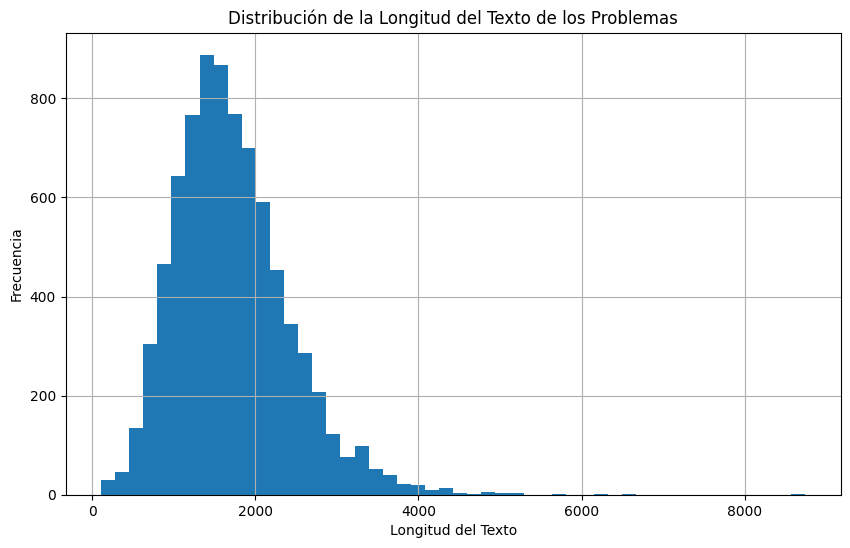
\includegraphics[scale=0.8]{imgs/len_description.png}
          \end{center}
          \newpage          
    \item Frecuencia de las etiquetas más comunes
          \begin{center}
              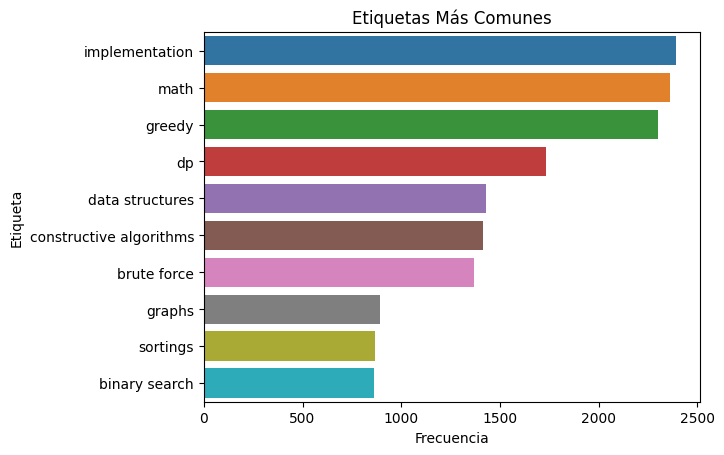
\includegraphics[scale=0.8]{imgs/common_tags_count.png}
          \end{center}
    \item Distribución de idiomas
          \begin{center}
              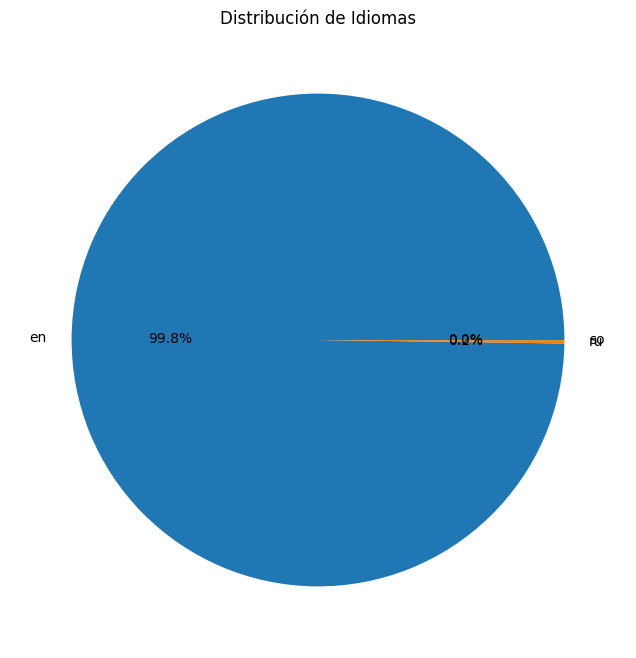
\includegraphics[scale=0.6]{imgs/langs_dist.png}
          \end{center}
          \newpage
          
    \item Nube de palabras asociada a la descripción de los problemas
          \begin{center}
              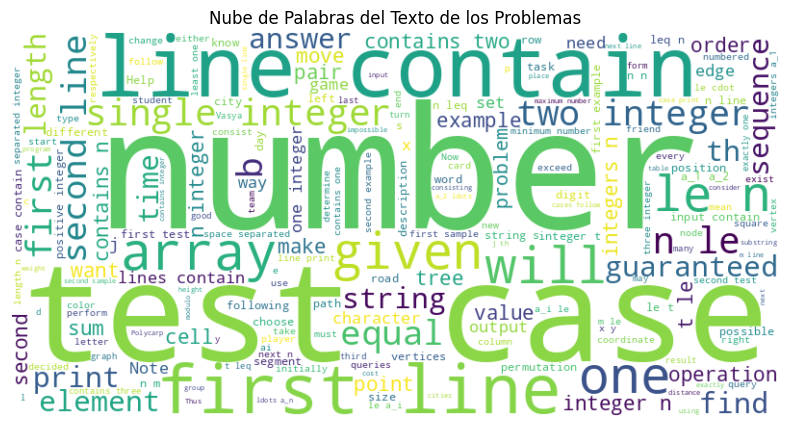
\includegraphics[scale=0.55]{imgs/wordcloud.png}
          \end{center}
    \item Matriz de correlación de las etiquetas
          \begin{center}
              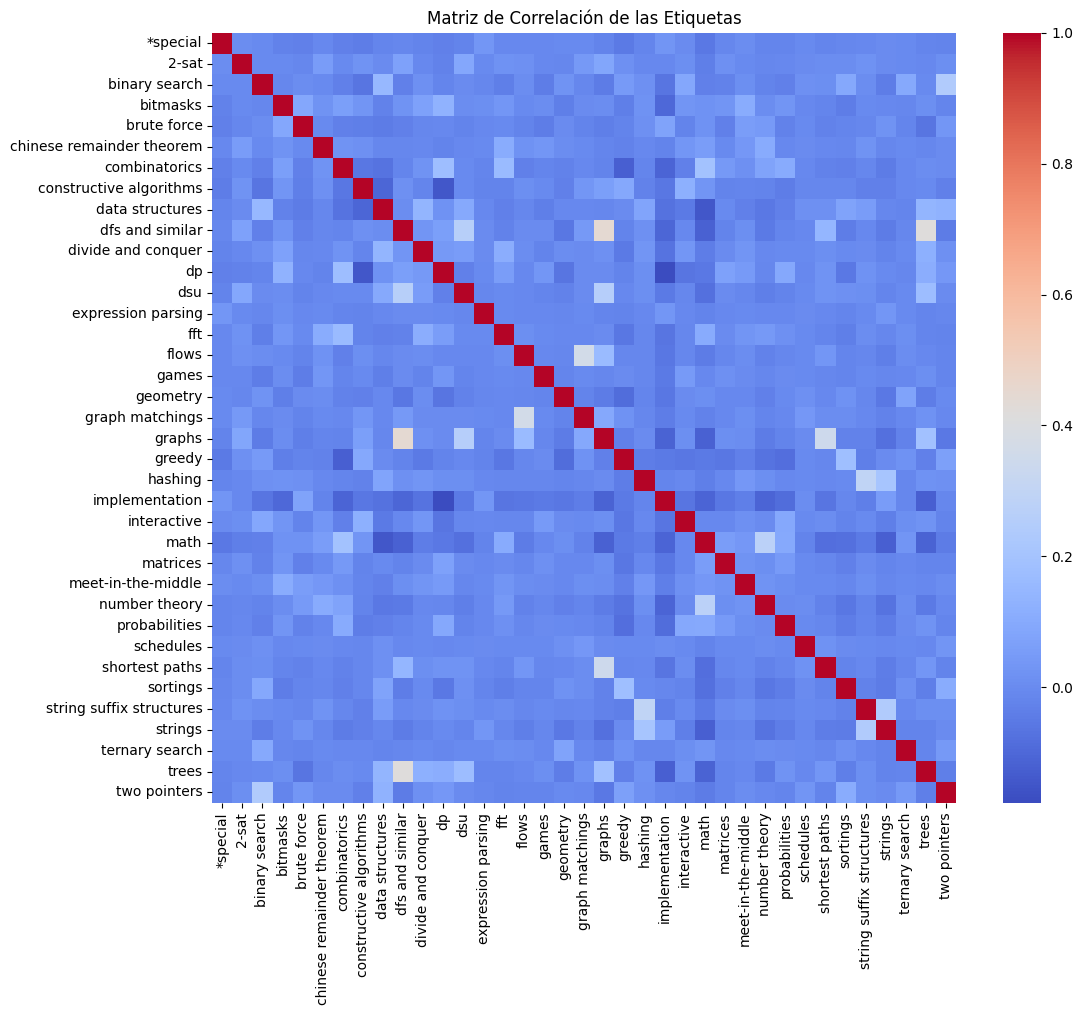
\includegraphics[scale=0.5]{imgs/correlation_matrix.png}
          \end{center}
\end{itemize}

\subsection{Preprocesamiento de datos}

\section{Estado del arte}

\subsection{Revisión bibliográfica}

En la revisión bibliográfica analizado encontramos 2 líneas de investigación fundamentales, modelos que analizaban solo
el lenguaje natural y por otro lado modelos que se enfocaban análisis en el análisis de código (es decir dado el texto o el ast
de un código en un lenguaje específico daba como salida los tags asociados a dicho código). A continuación se relacionan los 
papers estudiados.

\begin{itemize}
    \item Preprocesamiento de Lenguaje Natural
          
          \begin{longtable}{|p{2cm}|p{0.8cm}|p{2cm}|p{2cm}|p{3cm}|p{2cm}|p{3cm}|}
              \hline
              \textbf{Paper} & \textbf{Year}                                                                                                                                                       & \textbf{Link} & \textbf{Models} & \textbf{Results} & \textbf{Dataset} & \textbf{Methods} \\
              \hline
              \endfirsthead
              
              \hline
              \endfoot
              
              \hline
              \endlastfoot
              
              
              Predicting algorithmic approach for programming problems from natural language problem description 
                             & 2016 
                             & \href{https://ashishbora.github.io/assets/projects/nlp/report.pdf}{\url{https://ashishbora.github.io/assets/projects/nlp/report.pdf}}

              
              
              
              
              
                             & Long Short Term Memory (LSTM), Random Forest, dummy classifier 
                             & Only Random Forest outperformed the dummy classifier, which predicted the most popular class 
                             & Codeforces, considering only the first tag for each problem 
                             & Pre-trained word2vec vectors and one-hot encoding for input data representation                                                                                                                                                                                \\
              
              \hline
              Predicting algorithm classes for programming word problems
                             & 2019
                             & \href{https://aclanthology.org/D19-5511/}{\url{https://aclanthology.org/D19-5511/}}

              
              
              
              
              
                             & Convolutional Neural Networks (CNN), ensemble of CNNs, human predictors 
                             & Best results by ensemble of CNNs; human predictors had better results than the best model but with an F1-macro score of 0.43 on top-20 multi-label classification 
                             & Codeforces, predicting 10 and 20 most frequent tags 
                             & Multi-class and multi-label classification approaches for tag prediction                                                                                                                                                                                       \\
              
              \hline
              Multi-label classification for automatic tag prediction in the context of programming challenges
                             & 2019
                             & \href{https://arxiv.org/abs/1911.12224}{\url{https://arxiv.org/abs/1911.12224}}

              
              
              
              
              
                             & Long Short Term Memory (LSTM)
                             & Best F1 score by LSTM over one-hot encoding; best Weighted Hamming Score by LSTM over word2vec 
                             & Codeforces and TopCoder, tags sorted into 9 classes 
                             & Doc2Vec, LSTM over word2vec, LSTM over one-hot encoding                                                                                                                                                                                                        \\
              
              \hline
              Classification of Programming Problems based on Topic Modeling
                             & 2019
                             & \href{https://dl.acm.org/doi/10.1145/3323771.3323795}{\url{https://dl.acm.org/doi/10.1145/3323771.3323795}}

              
              
              
              
              
                             & k-Nearest Neighbors (kNN), Random Forest (RF), Multinomial Naive Bayes (MNB), Multilayer Perceptron (MLP) 
                             & Final accuracy did not improve much compared to TF-IDF baseline (0.86 vs 0.88 accuracy); positive impact on kNN and MNB, negative on RF 
                             & 
                             & Topic modeling (LDA, NMF) for vectorization; classification algorithms: kNN, RF, MNB, MLP                                                                                                                                                                      \\
              
              \hline
              
          \end{longtable}
          
    \item Análisis de Código
          
          \begin{longtable}{|p{2cm}|p{0.8cm}|p{2cm}|p{2cm}|p{3cm}|p{2cm}|p{3cm}|}
              \hline
              \textbf{Paper} & \textbf{Year}                                                                                                                                                                                                                                                                                               & \textbf{Link} & \textbf{Models} & \textbf{Results} & \textbf{Dataset} & \textbf{Methods} \\
              \hline
              \endfirsthead
              
              \hline
              \endfoot
              
              \hline
              \endlastfoot
              
              
              Automatic algorithm recognition of source-code using machine
              learning
                             & 2017
                             & \href{https://www.semanticscholar.org/paper/Automatic_Algorithm_Recognition_of_Source_Code_Shalaby_Mehrez/641beb8d201a9bda_27dd0b5a7727116_cd47c7cb9}{\url{https://www.semanticscholar.org/paper/Automatic_Algorithm_Recognition_of_Source_Code_Shalaby_Mehrez/641beb8d201a9bda_27dd0b5a7727116_cd47c7cb9}}

              
              
              
              
              
                             & Traditional classification algorithms 
                             & Successful application of traditional classification algorithms and code metrics for classifying solutions 
                             & Codeforces 
                             & Metric-based approach to source code vectorization; 30 different software metrics (e.g., number of variables of specific types, lines of code, number of loops, number of nested loops)                                                                                                                                                                                                                \\
              
              \hline
              Classification and recommendation of competitive programming problems
              using CNN
                             & 2017
                             & \href{https://www.researchgate.net/publication/321868484_Classification_and_Recommendation_of_Competitive_Programming_Problems_Using_CNN}{\url{https://www.researchgate.net/publication/321868484_Classification_and_Recommendation_of_Competitive_Programming_Problems_Using_CNN}}

              
              
              
              
              
                             & CNN character-wise 
                             & Managed to classify solutions into four classes; combining information from all submitted solutions improved classification 
                             & Codeforces 
                             & Character-wise CNN; proposed combining information from classifications of individual solutions                                                                                                                                                                                                                                                                                                        \\
              
              \hline
              
          \end{longtable}
          
          
\end{itemize}

\section{Propuestas de solución}
\begin{itemize}
    \item Clasificación Multietiqueta con TF-IDF y Naive Bayes
\end{itemize}

\section{Experimentación y resultados}

\subsection{Clasificación Multietiqueta con TF-IDF y Naive Bayes}
\subsubsection{Introducción}
La clasificación multietiqueta es una variante de la clasificación en la que cada instancia puede pertenecer a múltiples clases simultáneamente. En este estudio, utilizamos la vectorización TF-IDF para la extracción de características y un clasificador Naive Bayes para la clasificación. El objetivo principal es evaluar el rendimiento del modelo en varias métricas de evaluación.
\subsubsection{Metodología}
\begin{itemize}
    \item Preprocesamiento de Datos
\end{itemize}
El conjunto de datos preprocesado pasa a utilizar la vectorización TF-IDF para convertir los datos de texto en características numéricas. Las etiquetas se transformaron a un vector binario utilizando \texttt{MultiLabelBinarizer} para adaptarse a la naturaleza multietiqueta del problema.

\begin{itemize}
    \item Entrenamiento del Modelo
\end{itemize}
La clasificación se realizó utilizando un clasificador Naive Bayes dentro de un marco One-vs-Rest. El conjunto de datos se dividió en conjuntos de entrenamiento y prueba utilizando una división 80-20. Una vez el modelo predecía habían problemas a los cuales no se les
asignaba ninguna etiqueta, cosa que no sucede en el codeforces, por lo cual se le hace asignar a dichos problemas la etiqueta más probable, garantizando así que todo problema contenga al menos una etiqueta.

\begin{lstlisting}[language=Python, caption=Naive Bayes]
vectorizer = TfidfVectorizer()
X = vectorizer.fit_transform(text_data)
mlb = MultiLabelBinarizer()
y = mlb.fit_transform(labels)

X_train, X_test, y_train, y_test = train_test_split(X, y, test_size=0.2, random_state=42)

clf = OneVsRestClassifier(MultinomialNB())
clf.fit(X_train, y_train)
y_pred = clf.predict(X_test)
\end{lstlisting}
\newpage
\subsubsection{Resultados}
\begin{itemize}
    \item Informe de Clasificación
\end{itemize}
\begin{lstlisting}[language=Python, caption=Informe de Clasificación]
    classification_report(y_test, y_pred, target_names=mlb.classes_)
\end{lstlisting}

\begin{tabular}{lrrrr}
    \toprule
    {}                     & precision & recall   & f1-score & support \\
    \midrule
    bruteforce             & 0.200000  & 0.016393 & 0.030303 & 61.0    \\
    constructivealgorithms & 0.500000  & 0.013699 & 0.026667 & 73.0    \\
    datastructures         & 1.000000  & 0.040816 & 0.078431 & 49.0    \\
    dfsandsimilar          & 0.000000  & 0.000000 & 0.000000 & 4.0     \\
    dp                     & 0.000000  & 0.000000 & 0.000000 & 50.0    \\
    geometry               & 1.000000  & 0.176471 & 0.300000 & 17.0    \\
    greedy                 & 0.522727  & 0.414414 & 0.462312 & 111.0   \\
    implementation         & 0.515789  & 0.690141 & 0.590361 & 142.0   \\
    math                   & 0.630435  & 0.287129 & 0.394558 & 101.0   \\
    strings                & 0.833333  & 0.370370 & 0.512821 & 27.0    \\
    \bottomrule
\end{tabular}

\begin{itemize}
    \item Accuracy
\end{itemize}
\begin{verbatim}
Overall Accuracy: 14.46\%
\end{verbatim}

\begin{itemize}
    \item Matriz de Confusión
\end{itemize}
Se tiene un {\href{https://github.com/ARJ-Code/codeforce-tag-predictor/blob/main/src/naive\%20bayes\%20model/naive-bayes-model.ipynb}{jupyter interactivo}} en el que se puede consultar la matriz de confusión para cada etiqueta 
\newpage
\begin{itemize}
    \item Precision ,F1-Score ,Recall y Support para cada etiqueta
\end{itemize}
\begin{figure}[H]
    \centering
    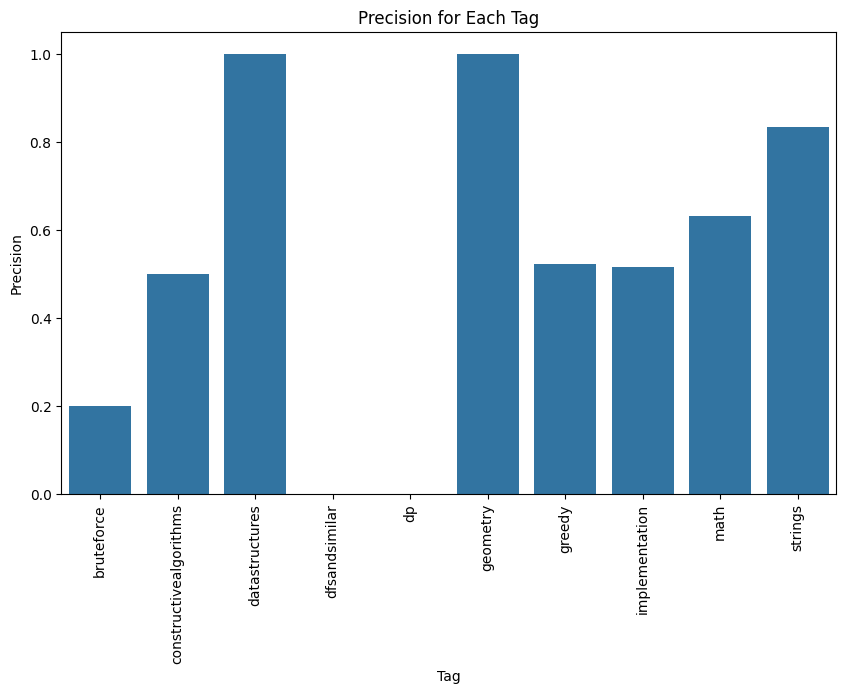
\includegraphics[scale=0.49]{imgs/precisonnb.png}
    \caption{Precision}
    \label{fig:p}
\end{figure}
\begin{figure}[H]
    \centering
    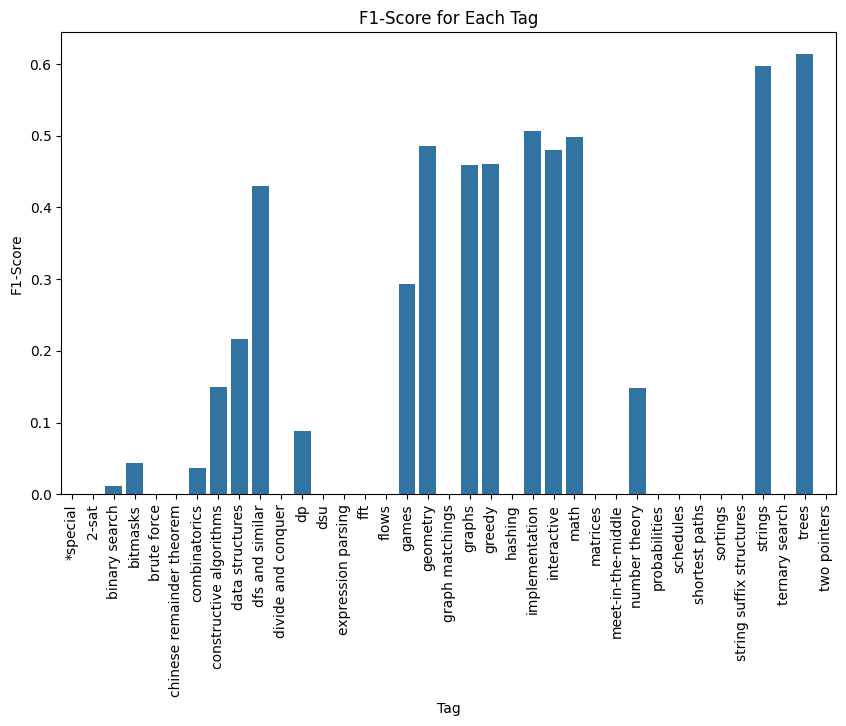
\includegraphics[scale=0.49]{imgs/f1nb.png}
    \caption{F1-Score}
    \label{fig:f1}
\end{figure}
\begin{figure}[H]
    \centering
    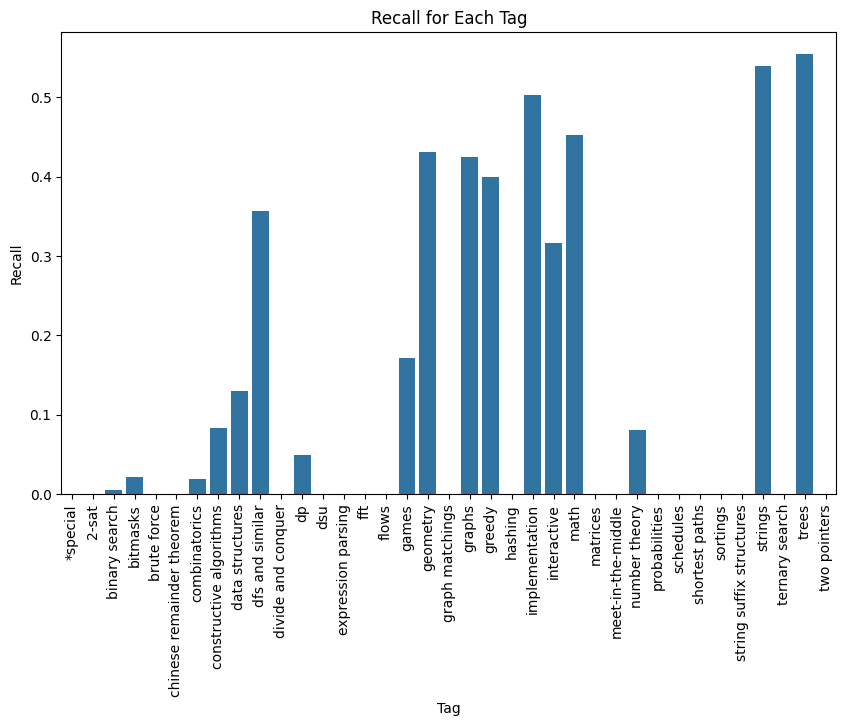
\includegraphics[scale=0.49]{imgs/recallnb.png}
    \caption{Recall}
    \label{fig:r}
\end{figure}
\begin{figure}[H]
    \centering
    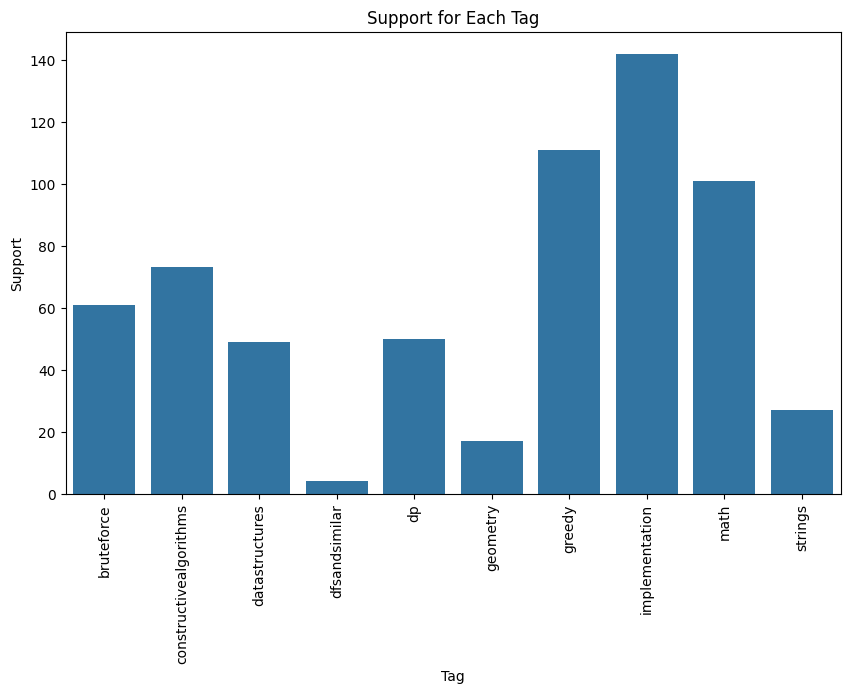
\includegraphics[scale=0.49]{imgs/supportnb.png}
    \caption{Support}
    \label{fig:s}
\end{figure}

\subsection{Clasificación Multietiqueta con TF-IDF y KNN}

\subsubsection{Introducción}
Al igual que en la sección anterior, usaremos el enfoque de modelo de aprendizaje multietiquetas. La vectorización usada es la misma que en Naive-Bayes, TF-IDF para extraer características y un clasificador KNN para la clasificación. El objetivo poder comparar el rendimiento de este modelo con los otros que hemos usado.

\subsubsection{Metodología}
\begin{itemize}
    \item Preprocesamiento de Datos
\end{itemize}
además de preprocesar la descripción de los problemas para usar TF-IDF, al ser KNN un modelo que solo se puede entrenar con valores numéricos, también se binarizaron los tags de los problemas, y se eliminaron columnas poco relevantes como el idioma y la identificación de los problemas.

\begin{itemize}
    \item Entrenamiento del Modelo
\end{itemize}
La clasificación se realizó utilizando un clasificador KNN dentro de un marco MultiOutput. El conjunto de datos se dividió en conjuntos de entrenamiento y prueba utilizando una división 80-20.\\ 
Pero cuál sería el mejor valor de K para el modelo, para esto se realizó una búsqueda de hiperparámetros con valores de K de 1 a 100, dando como resultado que K = 12 era el valor con mayor precisión en los resultados.

\begin{lstlisting}[language=Python, caption=KNN]
    
    X_train, X_test, y_train, y_test = train_test_split(X, y, test_size=0.2, random_state=42)
    
    neighbors = np.arange(1, 100)
    train_accuracies = {}
    test_accuracies = {}
    reports = []
    for neighbor in neighbors:
        knn = KNeighborsClassifier(n_neighbors=neighbor)
        mlb_knn = MultiOutputClassifier(knn)
        mlb_knn.fit(X_train, y_train)
        ypred = mlb_knn.predict(X_test) 
        train_accuracies[neighbor] = mlb_knn.score(X_train, y_train)
        test_accuracies[neighbor] = mlb_knn.score(X_test, y_test)
        reports.append(classification_report(y_test, ypred, zero_division = 0))
    \end{lstlisting}

\subsubsection{Resultados}
\begin{itemize}
    \item Informe de Clasificación
\end{itemize}

\begin{verbatim}
report = classification_report(y_test, y_pred, target_names=list(all_tags))
\end{verbatim}

\begin{tabular}{lrrrr}
    \toprule
                           & precision & recall   & f1-score & support    \\
    \midrule
    math                   & 0.410256  & 0.163265 & 0.233577 & 98.000000  \\
    strings                & 0.555556  & 0.500000 & 0.526316 & 30.000000  \\
    datastructures         & 0.900000  & 0.209302 & 0.339623 & 43.000000  \\
    greedy                 & 0.500000  & 0.350000 & 0.411765 & 100.000000 \\
    dfsandsimilar          & 0.000000  & 0.000000 & 0.000000 & 10.000000  \\
    constructivealgorithms & 0.100000  & 0.017544 & 0.029851 & 57.000000  \\
    implementation         & 0.602740  & 0.325926 & 0.423077 & 135.000000 \\
    geometry               & 1.000000  & 0.062500 & 0.117647 & 16.000000  \\
    bruteforce             & 0.500000  & 0.015152 & 0.029412 & 66.000000  \\
    dp                     & 0.000000  & 0.000000 & 0.000000 & 47.000000  \\
    \bottomrule
\end{tabular}

\begin{itemize}
    \item Accuracy
\end{itemize}
\begin{verbatim}
Overall Accuracy: 8.00\%
\end{verbatim}

\newpage
\begin{itemize}
    \item Precision ,F1-Score ,Recall y Support para cada etiqueta
\end{itemize}
\begin{figure}[H]
    \centering
    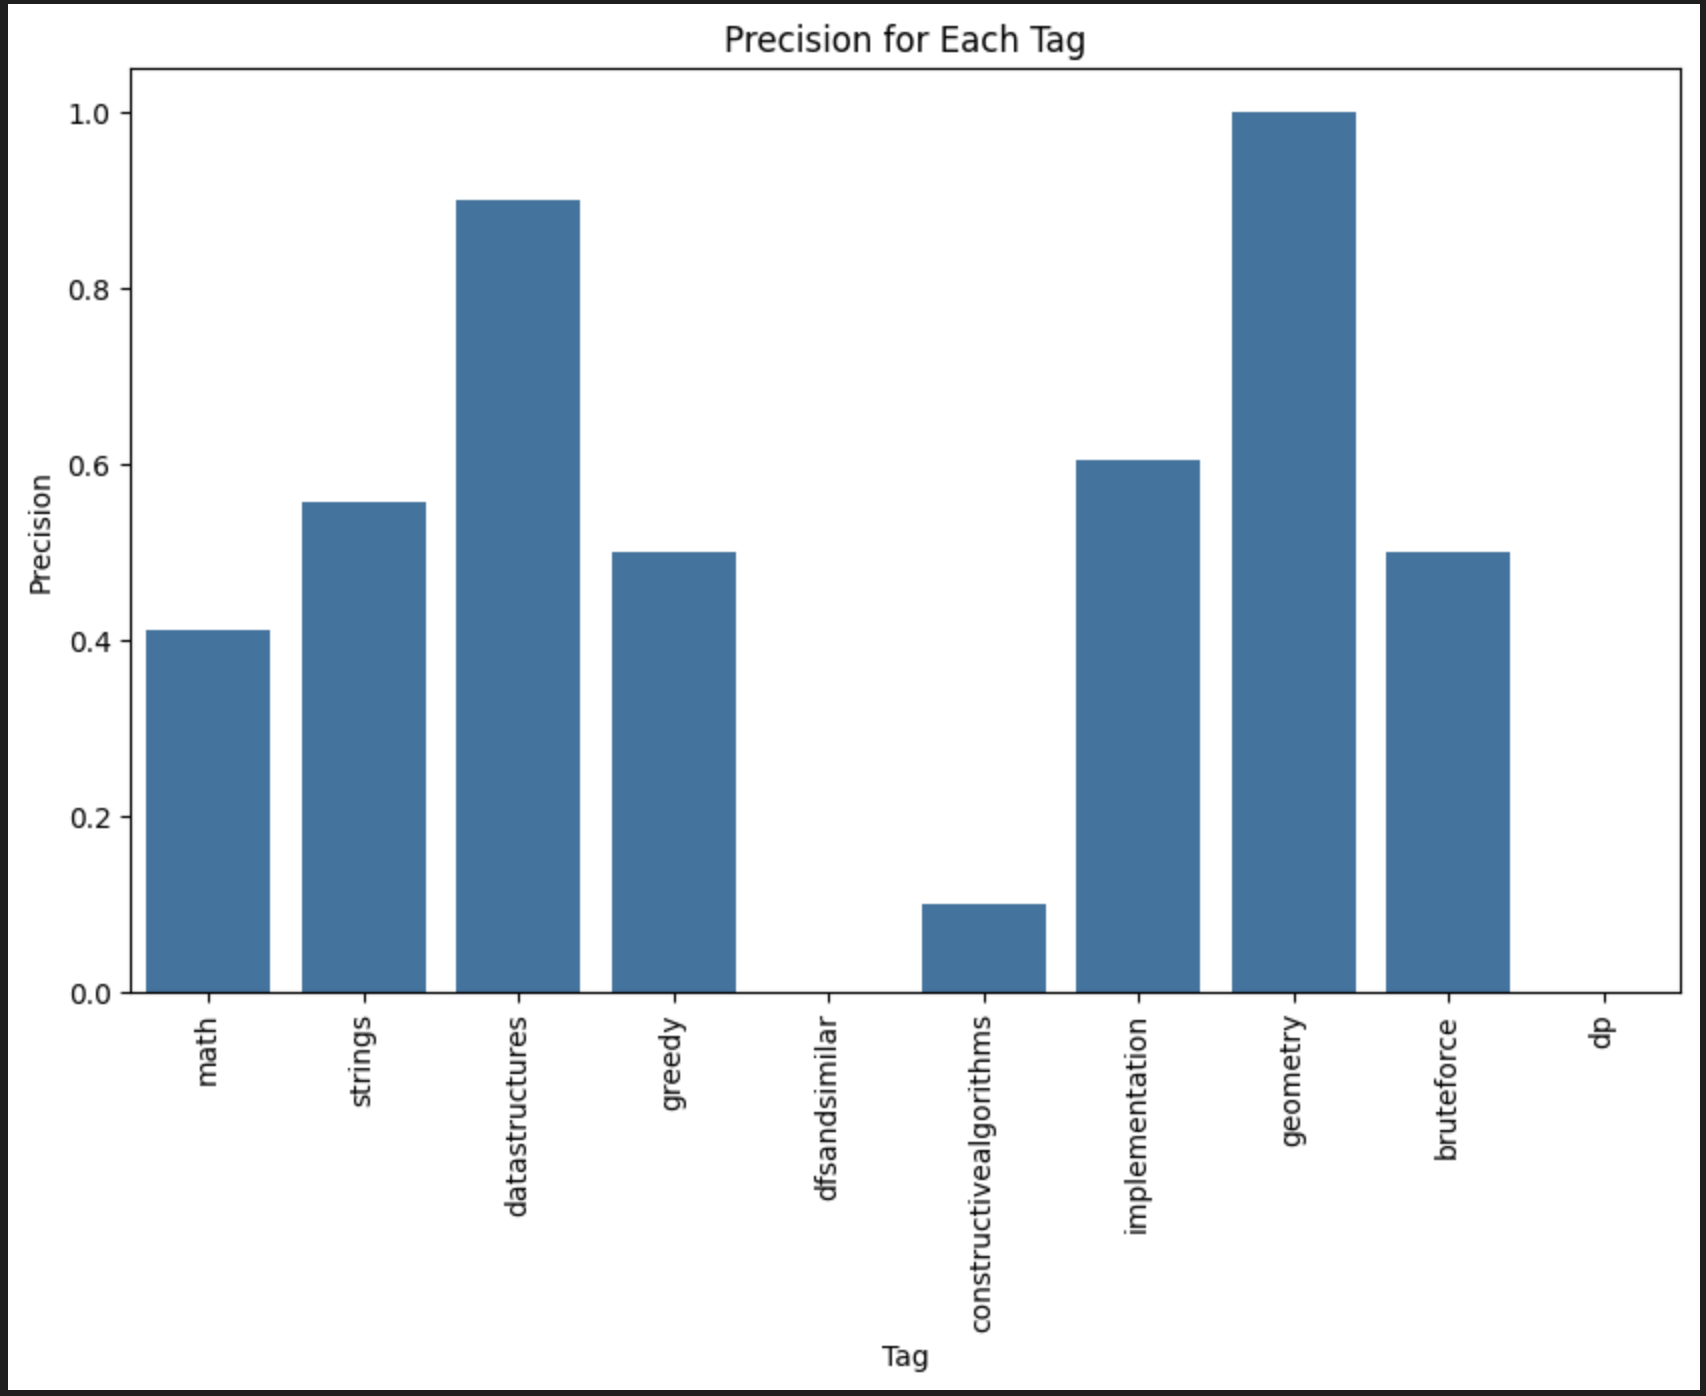
\includegraphics[scale=0.49]{imgs/precisonknn.png}
    \caption{Precision}
    \label{fig:p}
\end{figure}
\begin{figure}[H]
    \centering
    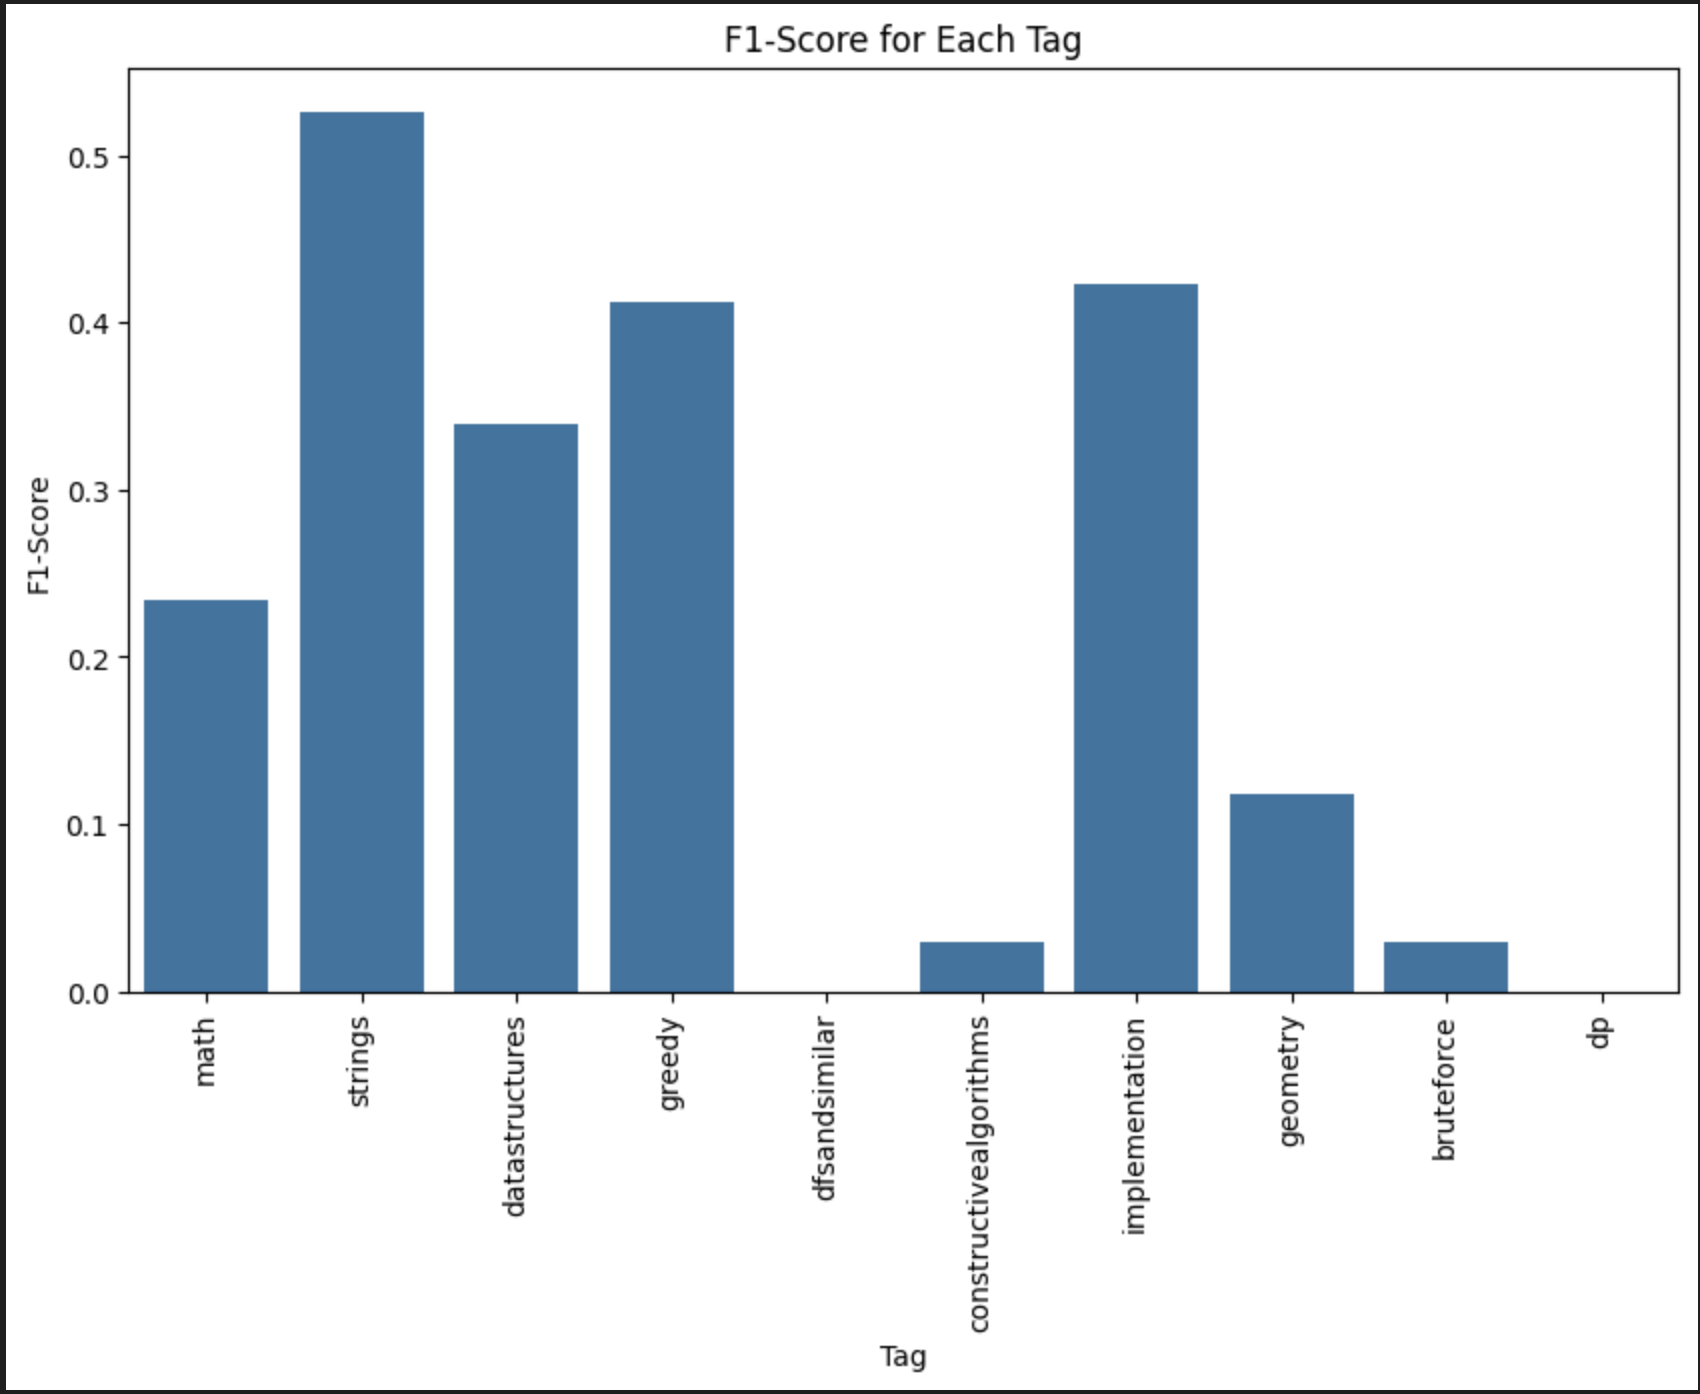
\includegraphics[scale=0.49]{imgs/f1knn.png}
    \caption{F1-Score}
    \label{fig:f1}
\end{figure}
\begin{figure}[H]
    \centering
    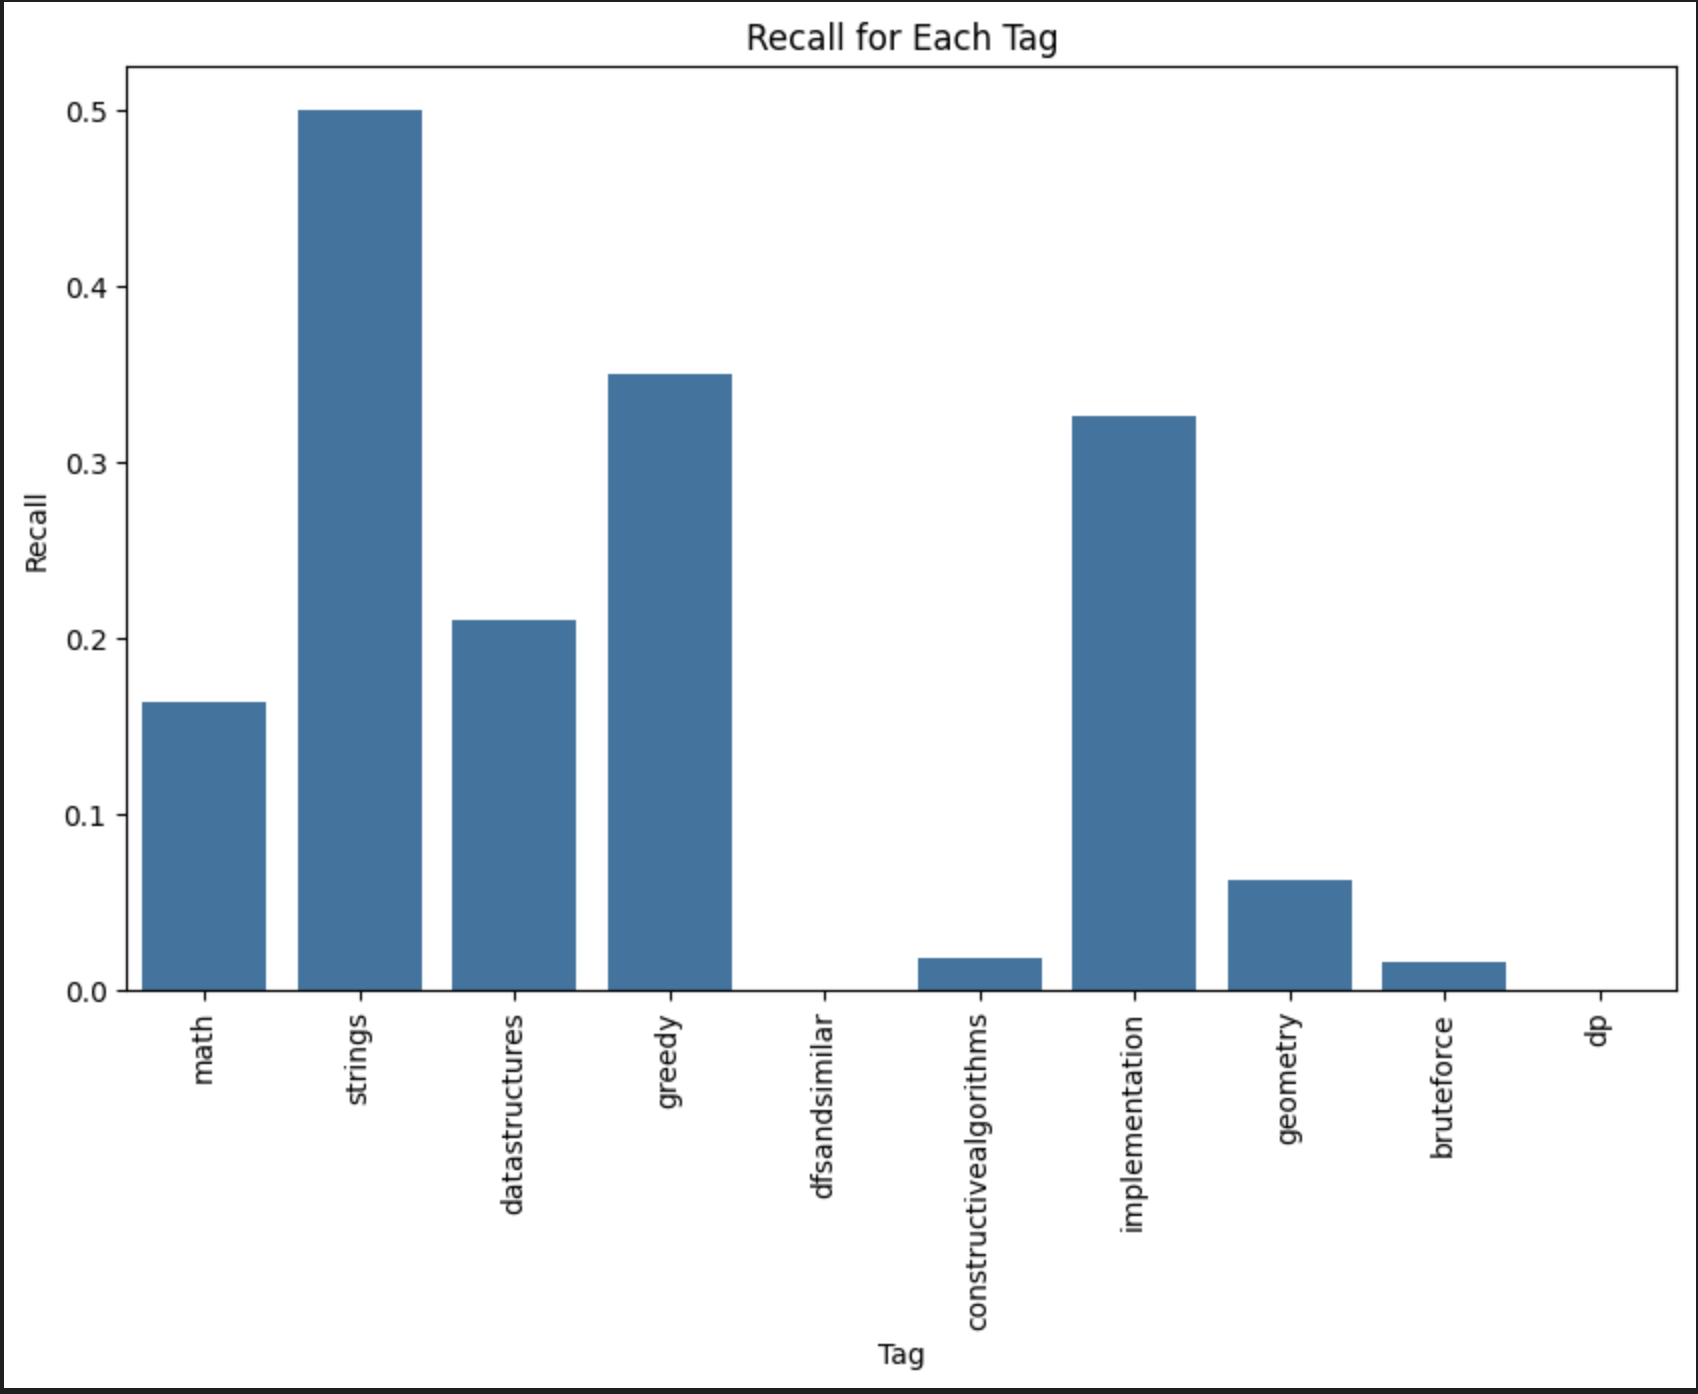
\includegraphics[scale=0.49]{imgs/recallknn.png}
    \caption{Recall}
    \label{fig:r}
\end{figure}
\begin{figure}[H]
    \centering
    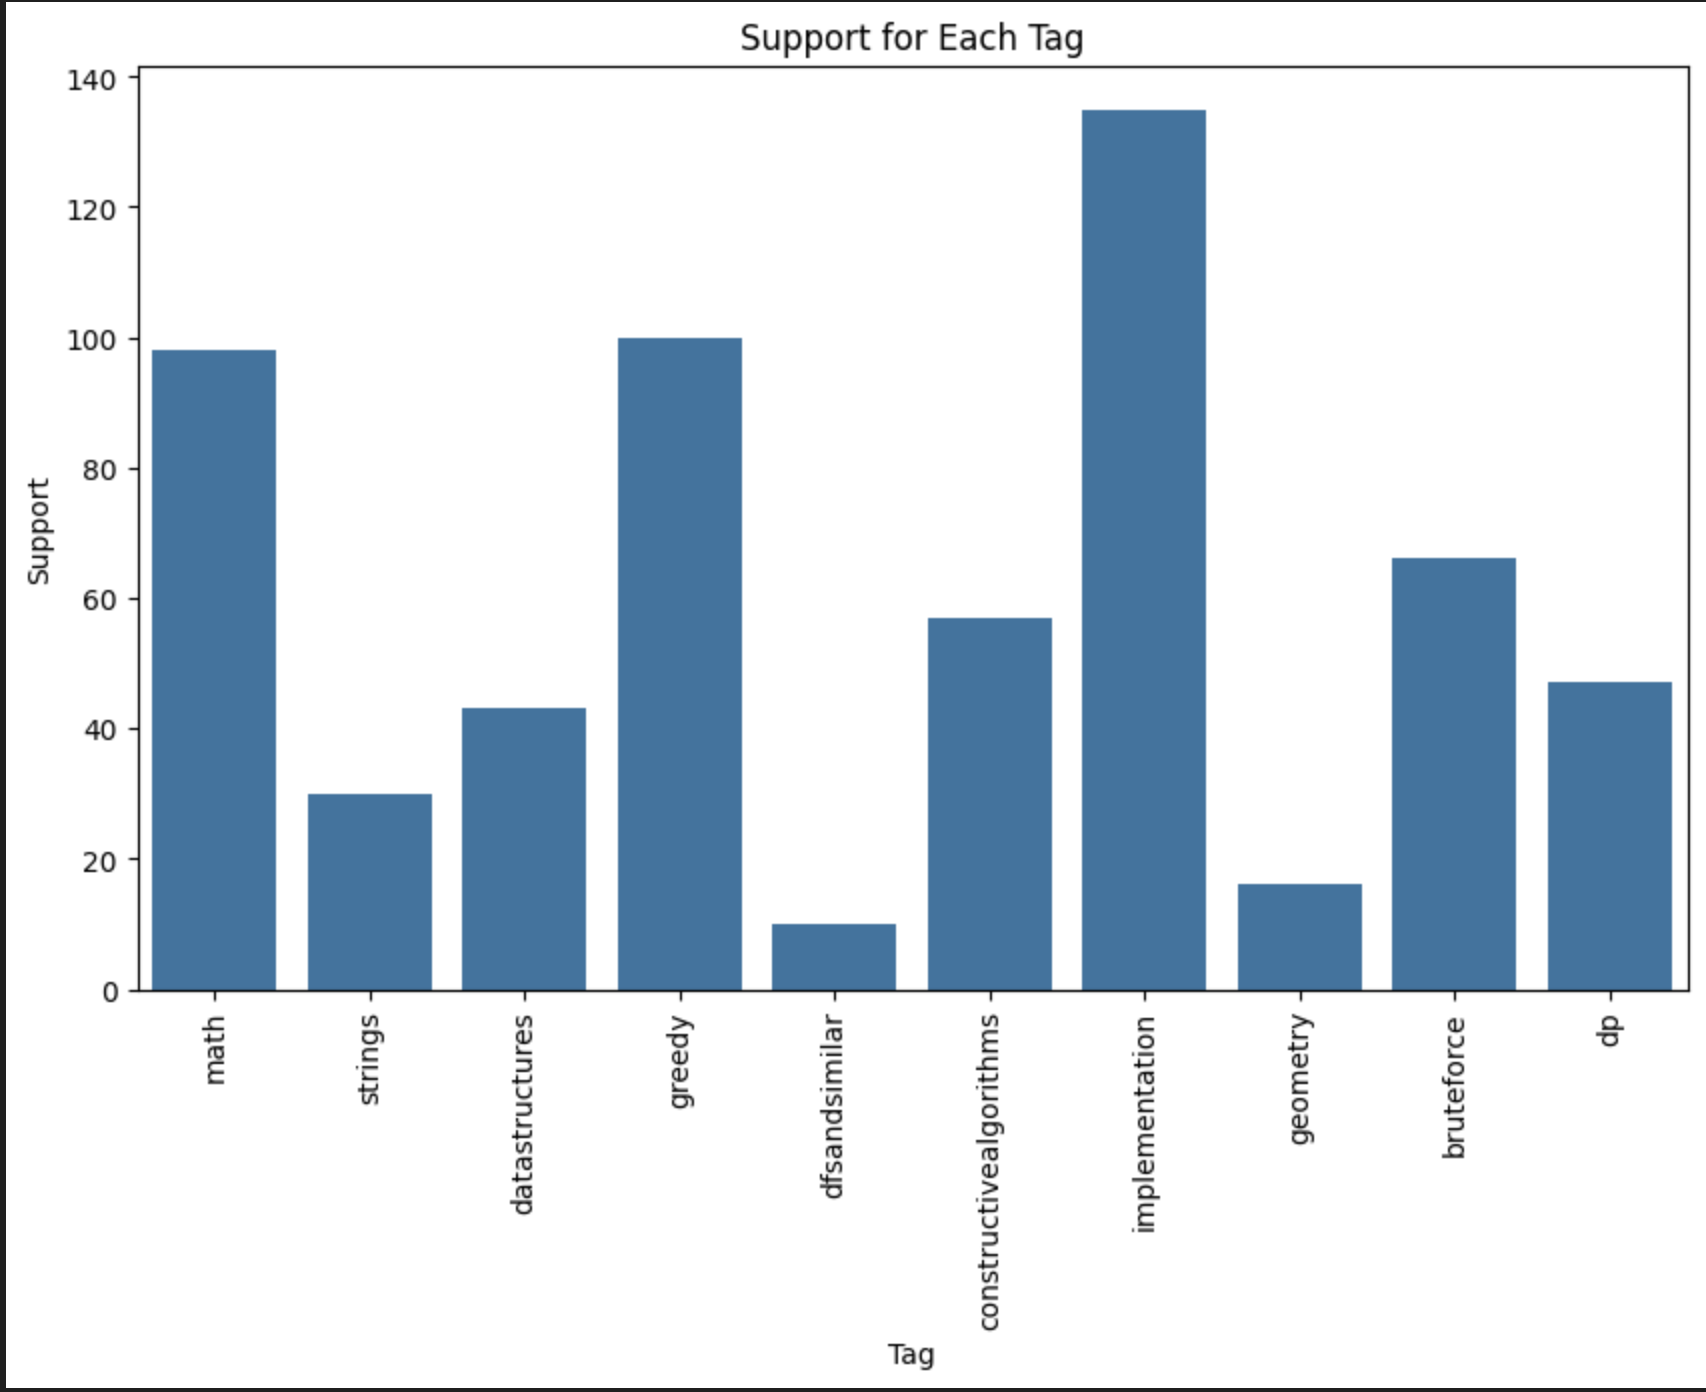
\includegraphics[scale=0.49]{imgs/supportkn.png}
    \caption{Support}
    \label{fig:s}
\end{figure}

\subsection{Chat GPT}

Para analizar que tan bien se comportaba Chat GPT 3.5, prediciendo los tags de Codeforces, usamos prompt engineering
con un preprocesamiento sobre los problemas:

\begin{lstlisting}[language=Python, caption=Prompt para tagear los problemas]
def prompt(description):
    all_tags_str = ', '.join(all_tags)
    return f'Give this set of {all_tags_str} tags and this problem ${description}, give me the set of problem tags in the following format: greedy, implementation, dp'
\end{lstlisting}

\begin{tabular}{|l|l|r|r|r|}
    \toprule
    {} & Metric        & ChatGPT  & Naive Bayes & KNN      \\
    \midrule
    0  & Accuracy      & 0.020000 & 0.146000    & 0.080000 \\
    1  & F1 (macro)    & 0.002431 & 0.240000    & 0.210000 \\
    2  & F1 (micro)    & 0.020000 & 0.390000    & 0.290000 \\
    3  & F1 (weighted) & 0.017556 & 0.320000    & 0.260000 \\
    4  & F1 (samples)  & 0.002431 & 0.390000    & 0.240000 \\
    \bottomrule
\end{tabular}

En el resto de los modelos comparados se obtuvieron mejores métricas en general, también vale destacar que no nos fue posible
usar ChatGPT 4o, modelo de mayor complejidad con le que esperamos que se comporte mejor, además de que solo nos fue posible 
analizar con ChatGPT 100 problemas ya que no disponíamos de la api y todo el trabajo se realizo de manera manual. Otro aspecto
a destacar, fue que en la mayoría de los problemas ChatGPT respondió  con los tags que se le mostraban de ejemplo en el prompt
lo que en alguna medida demuestra que el modelo en alguno o la mayoría de los casos alucinaba, algo que es común en estos modelos 
de lenguaje.

\section{Discusión de los resultados}
Primeramente señalar que como repercusión ética este trabajo puede ser maliciosamente utilizado en concursos online de 
programación competitiva, donde se tiene tolerancia cero al fraude tagueando los problemas 
y de esta manera saber con que idea atacar, aunque cabe destacar que los problemas usualmente no son tan triviales. También positivamente este trabajo es una excelente forma de que en la preparación individual en vista a competencias se pueda utilizar para solo concentrarse en problemas que tengan una etiqueta específica, además creemos que los modelos están abiertos a problemas no solo del propio codeforce, sino de otras plataformas de programación competitiva. Las ideas abordadas en el trabajo
estarán en disposición de todo aquel que quiera seguir avanzando con el tema en cuestión.

\section{Conclusiones y trabajo futuro}


\end{document}